\documentclass{beamer}
\usetheme{CambridgeUS}
\setbeamercovered{transparent}
%\usetheme{Hannover}

%\usetheme{Copenhagen}
\usepackage{graphicx}
\usepackage[utf8]{inputenc}
\usepackage[english]{babel}
\usepackage{calc}
\usepackage{amsmath}
\DeclareMathAlphabet{\mathonebb}{U}{bbold}{m}{n}
\usepackage{verbatimbox}
\usepackage{verbatim}
\usepackage{moreverb}
\usepackage{eurosym}
\usepackage{verbatim}      
\usepackage{amsmath, amsthm}                             
 
\usepackage{latexsym}                               
\usepackage{amssymb}
\usepackage{tabularx}
\usepackage{setspace}
\usepackage{listings}
\usepackage{geometry}


\usepackage{listings}
\definecolor{dkgreen}{rgb}{0,0.4,0}
\definecolor{gray}{rgb}{0.5,0.5,0.5}
\definecolor{mauve}{rgb}{0.58,0,0.82}

\usepackage[lined]{algorithm2e}
\newcommand{\algorithmicrequire}{\textbf{Input:}}
\newcommand{\algorithmicensure}{\textbf{Output:}}
\newcommand{\sign}{\text{sign}}
\newcommand{\argmin}{\text{argmin}}
\newcommand{\Cut}{\text{Cut}}
\newcommand{\Vol}{\text{Vol}}
\newcommand{\RCut}{\text{RCut}}
\newcommand{\NCut}{\text{NCut}}
\newcommand{\NCC}{\text{NCC}}
\newcommand{\RCC}{\text{RCC}}
\newcommand{\one}{\ensuremath{\mathonebb{1}}}


\usepackage{array}
\newcolumntype{L}[1]{>{\raggedright\let\newline\\\arraybackslash\hspace{0pt}}m{#1}}
\newcolumntype{C}[1]{>{\centering\let\newline\\\arraybackslash\hspace{0pt}}m{#1}}
\newcolumntype{R}[1]{>{\raggedleft\let\newline\\\arraybackslash\hspace{0pt}}m{#1}}

\usepackage{xcoffins}
\NewCoffin\tablecoffin
\NewDocumentCommand\Vcentre{m}
  {%
    \SetHorizontalCoffin\tablecoffin{#1}%
    \TypesetCoffin\tablecoffin[l,vc]%
  }


\definecolor{dkyellow}{cmyk}{0, 0, 0.2, 0}
\lstset{
  language=R,                % the language of the code
  basicstyle= \footnotesize,      % the size of the fonts that are used for the code
  numbers=left,                   % where to put the line-numbers
  numberstyle=\tiny\color{gray},  % the style that is used for the line-numbers
  stepnumber=2,                   % the step between two line-numbers. If it's 1, each line 
                                  % will be numbered
  showspaces=false,               % show spaces adding particular underscores
  showtabs=false,                 % show tabs within strings adding particular underscores
  frame=single,                   % adds a frame around the code
  rulecolor=\color{black},        % if not set, the frame-color may be changed on line-breaks within not-black text (e.g. commens (green here))
  tabsize=2,                      % sets default tabsize to 2 spaces
  captionpos=b,                   % sets the caption-position to bottom
  breaklines=true,                % sets automatic line breaking
  breakatwhitespace=false,        % sets if automatic breaks should only happen at whitespace
  keywordstyle=\color{blue},      % keyword style
  commentstyle=\color{dkgreen},   % comment style
  stringstyle=\color{mauve},       % string literal style
  backgroundcolor=\color{white},      % choose the background color. You must add \usepackage{color}
}

\usepackage{array}
\newcolumntype{L}[1]{>{\raggedright\let\newline\\\arraybackslash\hspace{0pt}}m{#1}}
\newcolumntype{C}[1]{>{\centering\let\newline\\\arraybackslash\hspace{0pt}}m{#1}}
\newcolumntype{R}[1]{>{\raggedleft\let\newline\\\arraybackslash\hspace{0pt}}m{#1}}

\usepackage{blkarray}% http://ctan.org/pkg/blkarray
\newcommand{\matindex}[1]{\mbox{\scriptsize#1}}% Matrix index

\title{Cell cycle analysis by live imaging}

\author{Peter Naylor}

\date{Internship defense}

\AtBeginSection[]
{
  \begin{frame}<beamer>{Sommaire}
    \tableofcontents[currentsection,currentsubsection]
  \end{frame}
}

\begin{document}
\begin{frame}{Recycling the MitoCheck project}
The mitocheck dataset is a unique dataset with a chromosome marker (H2B-eGFP). 200 000 filmed loss of function experiments. Can we used this data set to study the non-mitotic cell cycle phases? Idealy we would use a replication marker (PCNA-mcherry) but it is absent here.
\begin{figure}[!ht]
\centering
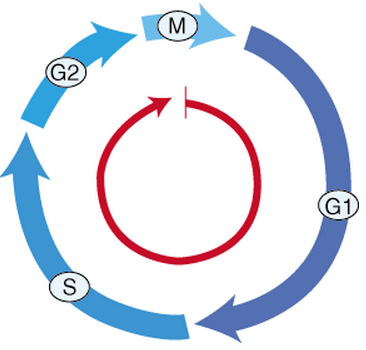
\includegraphics[width=0.3\textwidth]{Images/somaticcellcycle3.png}
\caption{Cell cycle}
\label{cellcycle}
\end{figure}

\end{frame}

\begin{frame}{The raw data}
\begin{columns}[T] % align columns
\begin{column}{.40\textwidth}
\begin{footnotesize}
\begin{figure}[!ht]
\centering
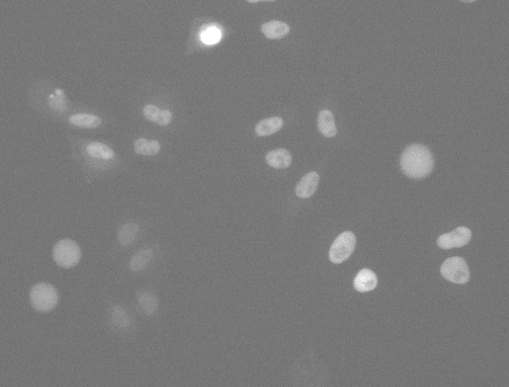
\includegraphics[width=0.50\textwidth]{Images/PCNA.png}
\caption{\textcolor{blue}{Figure :} Data acquired by Michael Olma with the \texttt{PCNA} marker}
\label{PCNA_michael_olma}
\end{figure}
\begin{itemize}
\item Data set that helps us label the data.
\item HeLa cells stably expressing \texttt{PCNA} marker which is informative about the non-mitotic phases.
\end{itemize}
\end{footnotesize}
\end{column}%
\hfill%
\begin{column}{.56\textwidth}
\begin{footnotesize}
\begin{figure}[!ht]
\centering
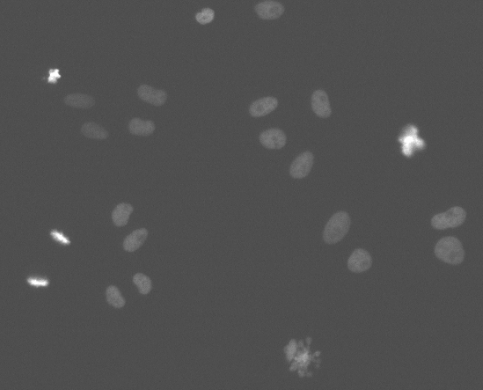
\includegraphics[width=0.38\textwidth]{Images/H2B.png}
\caption{\textcolor{blue}{Figure :} Data acquired by Michael Olma with the \texttt{H2B} marker}
\label{H2B}
\end{figure}
\begin{itemize}
\item Data set from which we extract features for training purposes. 
\item Looking for paterns that help differenciate non-mitotic phases.
\item HeLa cells stably expressing \texttt{H2B} marker, informative about the mitotic phases.
\end{itemize}
\end{footnotesize}
\end{column}%
\end{columns}
\end{frame}

\begin{frame}{Final Classifier}
\begin{figure}[!ht]
\centering
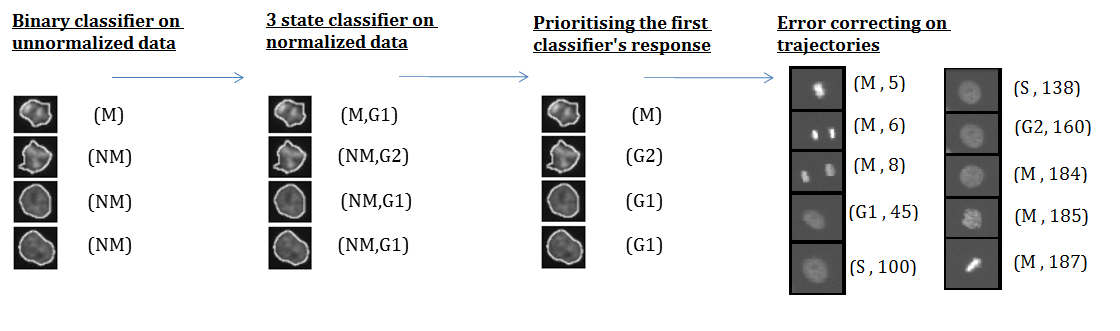
\includegraphics[width=\textwidth]{Images/Final_classif.png}
\caption{Final classifier (the error correcting model is missing).}
\label{Final_classifier}
\end{figure}
\end{frame}

\begin{frame}{Non-mitotic state classifier}
\begin{figure}[!ht]
\centering
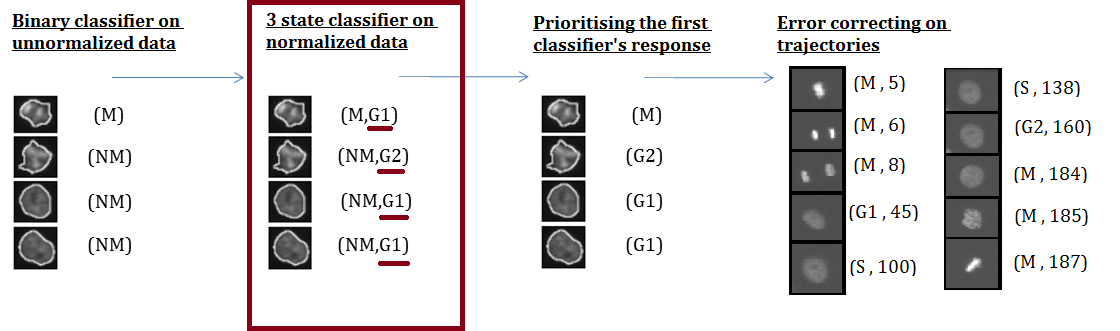
\includegraphics[width=\textwidth]{Images/First_part.png}
\caption{Non-mitotic state classifier}
\label{Non-mitotic state classifier}
\end{figure}
\end{frame}

\begin{frame}{Normalization process}
\begin{footnotesize}
Taking in account evolution of the cell with respect to time. Getting ride of cell-specific time invariant effects.

\begin{figure}[!ht]
\centering
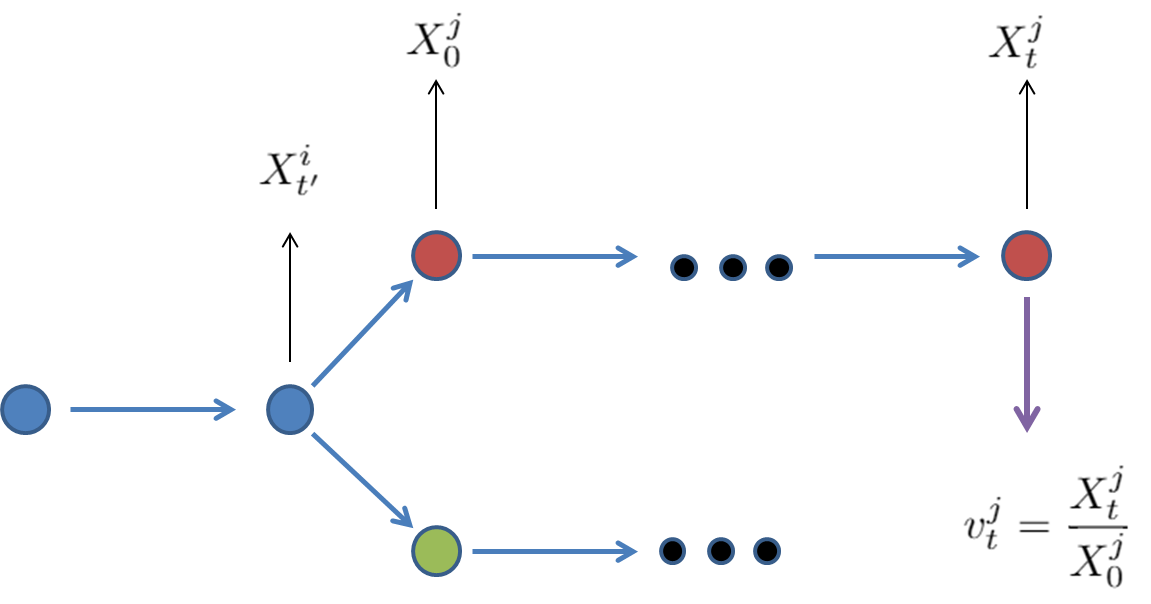
\includegraphics[width=0.4\textwidth]{Images/test1.png}
\caption{Normalisation of the data}
\label{normalization}
\end{figure}

Multiplicative model: the DNA is doubled, maybe the features double. Different normalization processes:
\begin{itemize}
\item Unnormalized: $v_t=X_t$: 0.72\%. 
\item Multiplicative with respect to the first moment after mitosis: $v_t=X_t/X_0$: 0.77\%.
\item Multiplicative with respect to all instances of the trajectory (like panel data):  $v_t=X_t/\bar{X}$: 0.72\%.
\item Additive with respect to the first moment after mitosis:  $v_t=X_t-X_0$: 0.77\%.
\item Additive with respect to all instances of the trajectory: $v_t=X_t-\bar{X}$: 0.72\%.
\end{itemize}
\end{footnotesize}
\end{frame}

\begin{frame}{Issues with the normalization process:}
\begin{itemize}
\item They are 1273 instances with labels.
\item Dividing with respect to $X_0$, bias procedure. Forces trajectories to have had a mitosis. Reduces number of labeled data to 508. In particular, only 37 labelled instances with Mitosis.
\item Averaging, can "destroy" the information, small trajectories. Filter by number of frames per trajectory? 
\item When dividing by $X_0$, we have to be careful, if $X_0$ contains 0's..
\end{itemize}
We also tried several models such as RandomForest, SVM with RBF kernel with different number of states:
\begin{itemize}
\item 2 states, S vs the rest.
\item G1, S and G2.
\item G1, S, G2 and M.
\end{itemize}
$\Longrightarrow$ Final model, 3 state classifier with division with respect to the first moment after mitosis.
 \end{frame}
 
\begin{frame}{Mitotic classifier}
\begin{figure}[!ht]
\centering
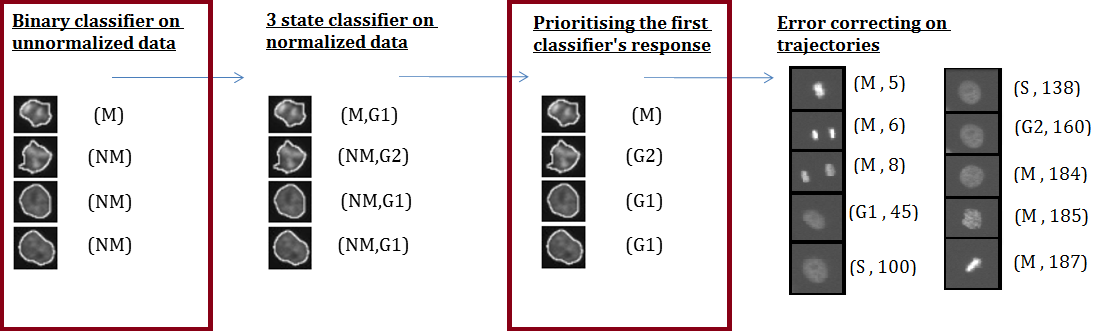
\includegraphics[width=\textwidth]{Images/Third_part.png}
\caption{Mitotic classifier}
\label{Mitotic classifier}
\end{figure}
\end{frame}

\begin{frame}{Mitotic classifier}
\begin{itemize}
\item Too few labelled mitosis, the classifier seemed unfit to predict mitosis events. 
\item We used the H2B channel with an unnormalized set to predict mitosis (accuracy above 90\%.) 
\item This classifier has priority over the 3 state classifier, if it predicts mitosis, then the cell will be in mitosis, if not it will be the prediction of the 3 state classifier.
\end{itemize}
\end{frame}


\begin{frame}{Hidden markov model}
\begin{figure}[!ht]
\centering
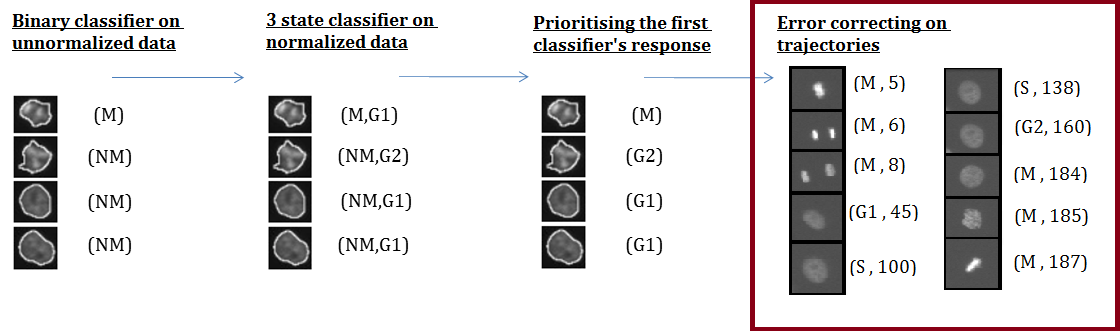
\includegraphics[width=\textwidth]{Images/Second_part.png}
\caption{Error correcting model}
\label{HMM_error}
\end{figure}
\end{frame}

\begin{frame}{Hidden Markov Model}
\begin{columns}[T] % align columns
\begin{column}{.48\textwidth}
\begin{figure}[!ht]
\centering
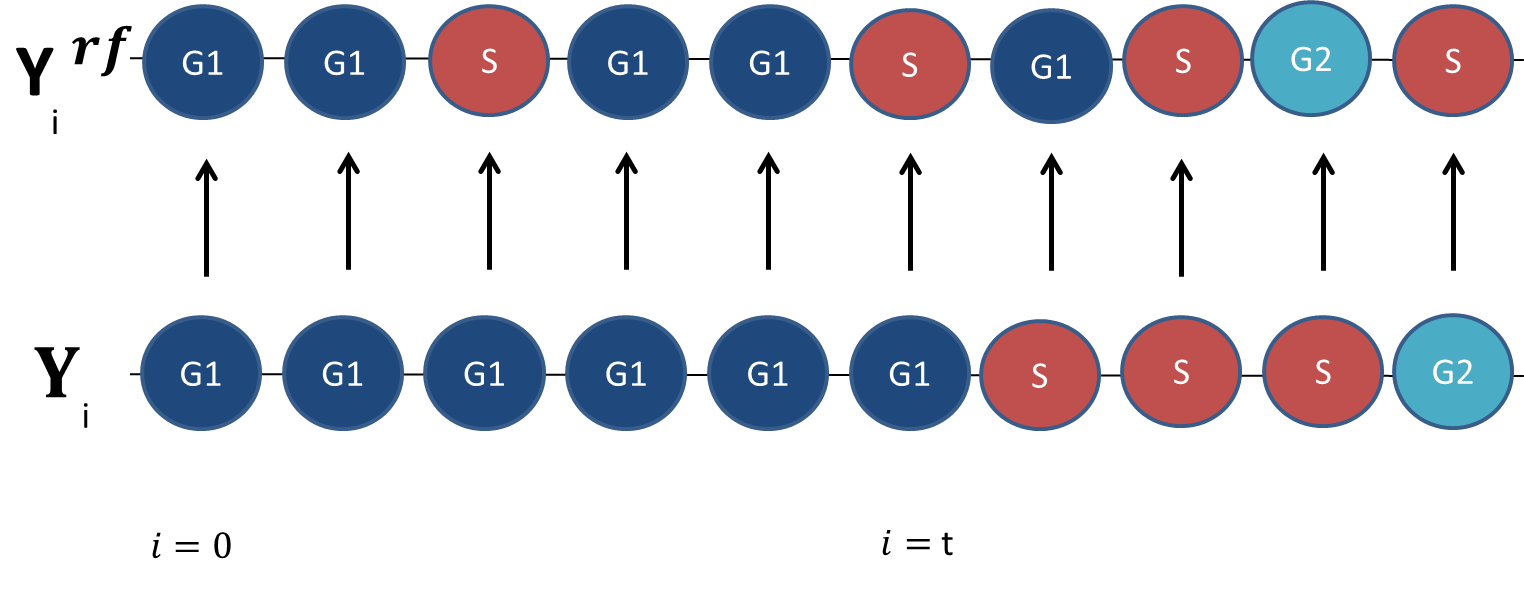
\includegraphics[width=0.95\textwidth]{Images/HMM.png}
%%\caption{Correcting a trajectory with the hidden markov chain}
\label{trajectory}
%%\textit{$Y^{rf}_i$ is the prediction of the cell at a certain frame $i$, $Y_i$ in its true state}
\end{figure}
\begin{figure}[!ht]
\centering
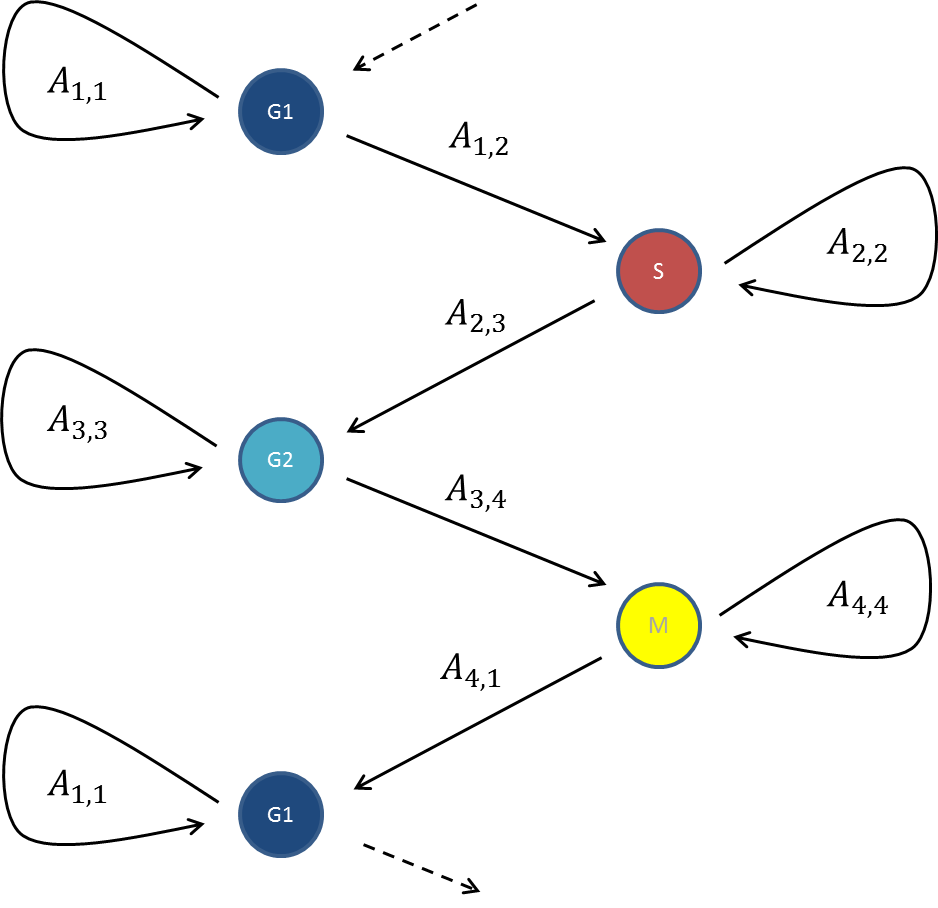
\includegraphics[width=0.6\textwidth]{Images/HMCmodel4.png}
\caption{ Hidden markov model}
\label{statetransition}
\end{figure}
\end{column}%
\hfill%
\begin{column}{.48\textwidth}
\begin{itemize}
\item Strong prior on the transition matrix.
\item Problem: Initial prediction of \textit{G2} is too poor. 
\item We reach an accuracy of 89\%, but without predictions of class \textit{G2}.
\item If we merge state \textit{S} and state \textit{G2} we reach 94\% accuracy.
\end{itemize}
\end{column}%
\end{columns}
\end{frame}

\begin{frame}{Issues with cyclic states}

\begin{columns}[T] % align columns
\begin{column}{.58\textwidth}
\begin{figure}[!ht]
\centering
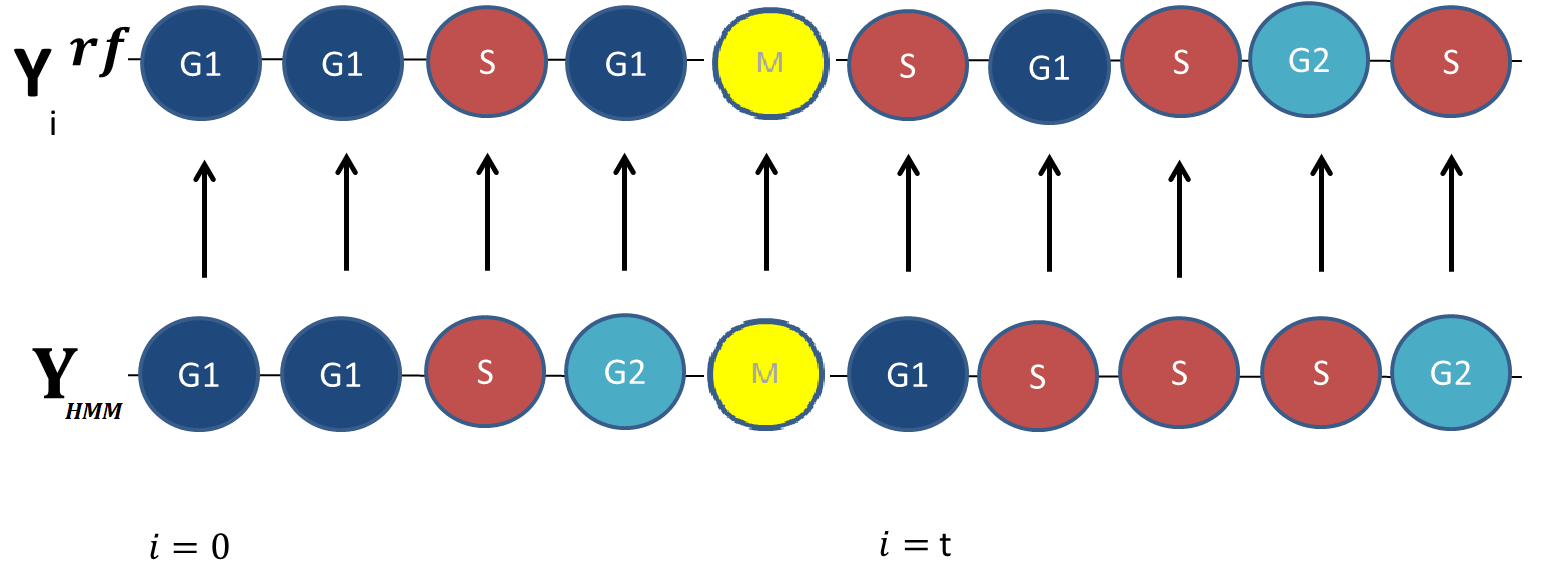
\includegraphics[width=1\textwidth]{Images/HMM_bad_correct.png}
\caption{Wrong correction}
\label{bad_correction}
\end{figure}
\end{column}%
\hfill%
\begin{column}{.38\textwidth}
\begin{figure}[!ht]
\centering
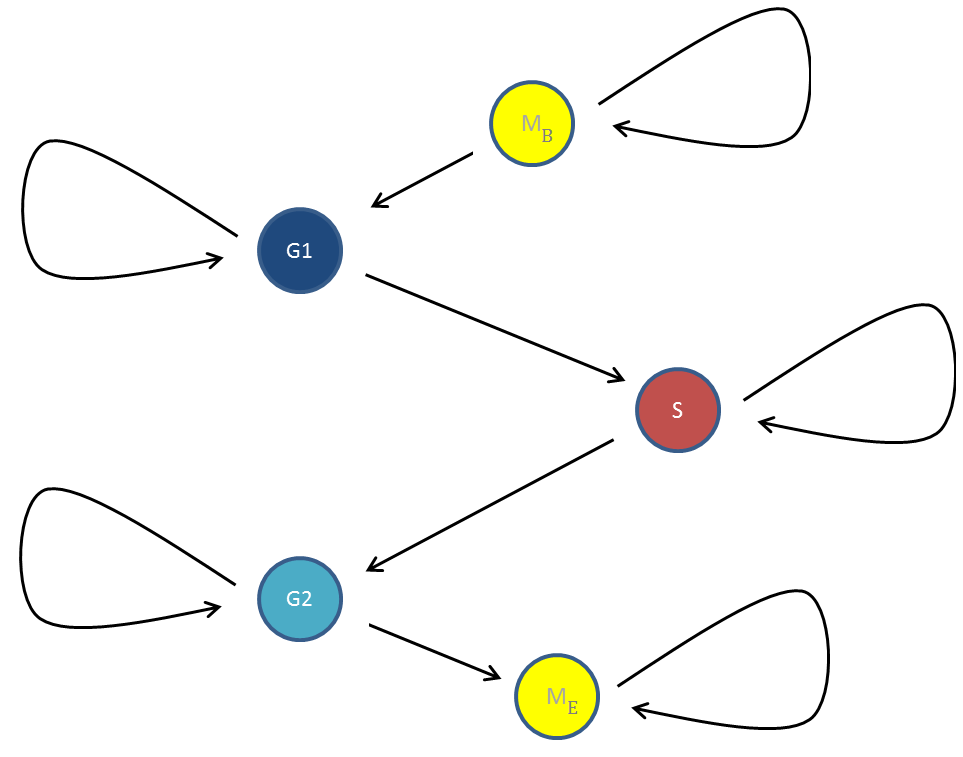
\includegraphics[width=1\textwidth]{Images/HMM5.png}
\caption{5 state hidden markov chain}
\label{trajectory_5}
%%\textit{$Y^{rf}_i$ is the prediction of the cell at a certain frame $i$, $Y_i$ in its true state}
\end{figure}
\end{column}%
\end{columns}
\begin{footnotesize}
\begin{itemize}
\item Sometimes, M is predicted in the middle of a trajectory (or maybe an other state, this can happen with states that have a good emission probability)
\item To stop it, we divide $M$ into $M_B$ and $M_E$. and change the state transition matrix, as above.
\end{itemize}
\end{footnotesize}
\end{frame}

\begin{frame}{Results on the cell cycle phases length}
\begin{footnotesize}
To assess our predicition, we looked at different cell cycle phases length out of 234 trajectories:
\begin{table}[!ht]
\centering
\begin{tabular}{|c|c|c|c|}
  \hline
  Length of:  & Mean & Standard deviation & Number of trajectories \\
  \hline
\text{G1} & 7.13 & 3.8 & 159 \\
  \hline
\text{S}  & 6.28 & 2.9 & 124 \\
  \hline
\text{G2} & 3.17 & 1.4 & 124 \\
  \hline
\text{Cell Cycle} & 16.7 & 4.1 & 124 \\
  \hline 
\end{tabular} 
  \caption{On Michael Olma set with the PCNA channel, our "ground truth"}
\end{table}
\begin{table}[!ht]
\begin{tabular}{|c|c|c|c|}
  \hline
  Length of:  & Mean & Standard deviation & Number of trajectories \\
  \hline
\text{G1} & 6.92 & 3.6 & 164 \\
  \hline
\text{S}  & 8.30 & 3.1 & 102 \\
  \hline
\text{G2} & 1.77 & 2.2 & 102 \\
  \hline
\text{Cell Cycle} & 17.1 & 2.1 & 102 \\
  \hline 
\end{tabular} 
  \caption{On Michael Olma set with the H2B channel}
\end{table}
\end{footnotesize}
\end{frame}

\begin{frame}{Results on MitoCheck dataset}
\begin{footnotesize}
\begin{table}[!ht]
\centering
\begin{tabular}{|c|c|c|c|}
  \hline
  Length of:  & Mean & Standard deviation & Number of trajectories \\
  \hline
\text{G1} & 11.76 & 6.27 & 277 \\
  \hline
\text{S}  & 5.81 & 3.64 & 194 \\
  \hline
\text{G2} & 5.19 & 4.19 & 29 \\
  \hline
\text{Cell Cycle} & 23.00 & 3.94 & 29 \\
  \hline 
\end{tabular} 
  \caption{Basic characteristics of phases length on the MitoCheck data set out of 2408 trajectories.}
\end{table}
With KMM transfer learning:
\begin{table}[!ht]
\centering
\begin{tabular}{|c|c|c|c|}
  \hline
  Length of:  & Mean & Standard deviation & Number of trajectories \\
  \hline
\text{G1} & 12 & 6.5 & 343 \\
  \hline
\text{S}  & 5.8 & 3.9 & 252 \\
  \hline
\text{G2} & 5.4 & 5.1 & 108 \\
  \hline
\text{Cell Cycle} & 23.00 & 3.8 & 78 \\
  \hline 
\end{tabular} 
  \caption{Basic characteristics of phases length on the MitoCheck data set, with transfer learning (instance reweighting).}
\end{table}
\end{footnotesize}
\end{frame}

\begin{frame}{Further work}

\begin{itemize}
\item Acquiring more ground truth about the mito check dataset.
\item Filter the trajectories better, with respect to the number of frames in the trajectory or with a tighter score on the future of the trajectory.
\item Different transfer learning technic, such as feature transfer instead of instance reweighting.
\end{itemize}

\end{frame}

\end{document}